\documentclass[11pt]{article}
\usepackage[left=25mm, right=25mm, top=25mm, bottom=25mm, includehead=true, includefoot=true]{geometry}

\usepackage{graphicx}
\usepackage{url}
\usepackage{natbib} % For referencing
\usepackage{authblk} % For author lists
\usepackage[parfill]{parskip} % Line between paragraphs
\usepackage{wrapfig} % For wrapping text around tables / figures

\pagenumbering{gobble} % Turn off page numbers

% Make all headings the same size (11pt):
\usepackage{sectsty}
\sectionfont{\normalsize}
\subsectionfont{\normalsize}
\subsubsectionfont{\normalsize}
\paragraphfont{\normalsize}


\renewcommand{\abstractname}{Summary} % Make 'abstract' be called 'Summary'


% This makes links and bookmarks in the pdf output (should be last usepackage command because it overrides lots of other commands)
\usepackage[pdftex]{hyperref} 
\hypersetup{pdfborder={0 0 0} } % This turns off the stupid colourful border around links



% **************  TITLE AND AUTHOR INFORMATION **************

\title{A Global Analysis of Bus Route Structure}

\author[1,2]{Ed Manley\thanks{e.j.manley@leeds.ac.uk}}
\author[3]{Steven Gray}
\author[1,2]{Nick Malleson}
\affil[1]{School of Geography, University of Leeds}
\affil[2]{Leeds Institute for Data Analytics, University of Leeds}
\affil[3]{Centre for Advanced Spatial Analysis (CASA), University College London}

\renewcommand\Authands{ and } % correct last comma in author list

\begin{document}

\maketitle

% **************  ABSTRACT/SUMMARY  **************

\begin{abstract}
\centering

Bus networks serve a vital purpose in urban public transport, and ensuring accessibility to the bus service is an important transport planning duty for any city. However, we currently lack systematic approach to bus network analysis, that accounts for varying street network structures and city size. This paper introduces a methodology for a global analysis of bus network design. It uses General Transit Feed Specification (GTFS) data with freely available Open Street Map road network data to compare the features of the bus routes in different cities worldwide. Through clustering we are able to extract common trends in bus route design. Initial results demonstrate commonalities and differences between cities, and suggest that route network data holds promise as a means of estimating the quality of bus service provision.

$ $ \\ {\bf KEYWORDS:} Public Transportation; Bus Networks; Accessibility; Network Entropy; Clustering.

\end{abstract}

% **************  MAIN BODY OF THE PAPER **************

\section{Introduction}

The adequate provision of public transport, and local bus services in particular, has long been recognised as vital for a healthy society. For example, in the UK there is evidence that in many places people without cars face difficulties accessing essential services such as doctors' surgeries~\citep{lovett_car_2002} and shops~\citep{guy_food_2004, lucas_providing_2006}. These difficulties have been exacerbated by trends towards a greater reliance on car use at the expense of publicly-funded transport infrastructure, particularly in the 1970s and 1980s~\citep{higgs_changes_1997}, causing some people, particularly with low incomes in rural communities~\citep{lowe_deprivation_1986}, to face social exclusion~\citep{pooley_mobility_2016}.  In many places it has become ``virtually impossible'' to perform normal daily activities without access to a car~\citep{lucas_transport_2001} and this situation will only get worse as the age structures in industrialised countries moves towards a larger proportion of elderly people who (for a number of reasons) will not use cars~\citep{lucas_providing_2006}.

Previous attempts to measure accessibility and the impact of public transport provision include the use of the Public Transport Accessibility Level (PTAL) approach~\citep{wu_ptal_2003} and similar indices~\citep{currie_quantifying_2010, delbosc_using_2011} as well as equity measures such as the Gini coefficient and Lorenz curve~\citep{delbosc_using_2011} and neuanced calculations of the connectivity of each transit stop to the wider network~\citep{welch_measure_2013}. However, due to the difficulties in collecting, cleaning and analysing comparative data from large and diverse administrative areas, most previous studies focus solely on a sub-national regions. Although such regional analyses undoubtedly provide useful insights for their target areas, they prohibit analysis of wider (i.e. national) government policy or comparisons of different local authority regimes.

This preliminary study, instead, begins to use data from a number of different cities across the globe. Although the data are less rich than those that are often available at the regional level, the ability to compare public transport provision across different cities, let alone different countries, offers exciting opportunities for comparing how well different cities and countries serve their residents. This research collects data on bus routes from a total of 95 cities in 19 countries and calculates a number of different measures that characterise the structures of the bus bus routes. It then clusters the individual routes according to their similarity and explores the differences across cities. The results reveal high global variation in provision of different service types, primarily based on the proportions of `Express' routes designed into the network. Although the metrics currently preclude an overall assessment of \textit{accessibility}, the results highlight that the data and methods hold considerable potential for further global assessments of public service provision. Furthermore, by using publicly-available data and open source code, the work is entirely reproducible. 

% Table part of section 2 but included here so that it wraps properly
\begin{wraptable}{r}{0.5\textwidth}
	\centering
%	\vspace{-2cm}
	\begin{tabular}{ l r }
		\hline
		Country & Number of routes \\
		\hline
		USA         &        4601 \\
		Australia   &        1980 \\
		Canada      &        1789 \\
		Italy       &         853 \\
		New Zealand &         777 \\
		Russia      &         709 \\
		Finland     &         575 \\
		Hungary     &         365 \\
		Poland      &         356 \\
		Austria     &         354 \\
		Czechia     &         328 \\
		Spain       &         282 \\
		Lithuania   &         182 \\
		France      &         175 \\
		Germany     &         172 \\
		Mexico      &         119 \\
		\hline
	\end{tabular}
	\caption{The number of routes per country included in the analysis}	
	\vspace{-1.5cm} % tweak to correct the formatting
	\label{tab:num_cities}
\end{wraptable}

This paper has been structured as follows. Section~\ref{data_sources} outlines the data sources used, Section~\ref{clustering} presents the details of the analysis and clustering results, and Section~\ref{conclusion} draws conclusions.




\section{Data Sources}\label{data_sources}

The data was collected using a GTFS data service provided by OpenMobilityData (\url{transitfeeds.com}) which provides an updated API of various public transit data from transit authorities worldwide.  The service allows authenticated users, by way of an authentication key, to fetch data programmatically via the API and directly download the GTFS data that is collated by the service. In many cities there are multiple providers of transit data and as data is updated by these transit authorities on a regular basis a reproducible workflow has been created to fetch data from OpenMobilityData to collect the data into one large collection for analysis.

The workflow consists of various interconnected scripts which fetch and process the individual zip files for each transit authority for all the cities in the OpenMobilityData collection and creates an index for these downloaded files.  Each file has an associated checksum created within the workflow so that in future iterations of the workflow the data can be refreshed if there is an update to the source GTFS data. At this stage each zip file is unpacked, checked for validity and cleaned if any errors are found within the source file. The cleaned data, line by line is, inserted into a master file which after processing all of the collection is, in turn, inserted into a database for later analysis. This workflow results with a final collection of 3,337 agencies, 12.3 million routes consisting of 1.6 million stops.  

After data cleaning and removing circular routes, the analysis covers 95 cities in 19 countries. As might be expected, there is an over-representation of countries in the Global North and as illustrated in Table~\ref{tab:num_cities}. 

\section{Bus Route Clustering}\label{clustering}

After the GTFS data were downloaded, a number of metrics were calculated to describe the different characteristics of each bus route. Table~\ref{tab:cluster_features} outlines these features. All parameters measures are normalised by characteristics of the city or route structure. This ensures that we control for varying city size and street network arrangement, which naturally impact bus route design. These normalised measures should more closely reflect the relative route design preferences imposed by transport planners in each city. 

\begin{table}[ht]
\caption{Features of the bus routes used in the classification. All features are normalised by city or route features.}
\begin{center}
\begin{tabular}{c|p{0.7\textwidth}}
\hline 
Feature & Description \\
\hline 
Route Length & The length of the bus route, normalised by the maximum route length for all routes in the city that the route is part of \\ 
Stop Distance & Number of stops on route, normalised by route length \\
Sinuocity & Measure of actual the route length divided by the Euclidean distance between origin and destination \\
Curvature & Sum angular deviation of route normalised by relative entropy of city street network \citep{boeing_urban_2019} \\
Turns & The number of major turns (greater than 60 degrees), normalised by route length \\
\hline
\end{tabular}
\end{center}
\label{tab:cluster_features}
\end{table}%

K-Means clustering is a commonly used approach and is appropriate here as a means of clustering the bus routes according to the similarities of the features outlined in Table~\ref{tab:cluster_features}. Before running the analysis, however, an appropriate number of clusters used must be determined. If there are too many clusters then similar routes will not be grouped together, whereas using too few clusters risks creating overlapping clusters. The Silhouette Coefficient, $S$, can be used to determine the most appropriate number of clusters. $S$ is a measure of the mean distances that each bus route is from its constituent cluster centroid. Values of 1 indicate that all routes are close to their assigned cluster and values of 0 suggest that there are overlapping clusters. 

\begin{figure}[ht] \begin{center} 
\resizebox{0.9\textwidth}{!}{ 
	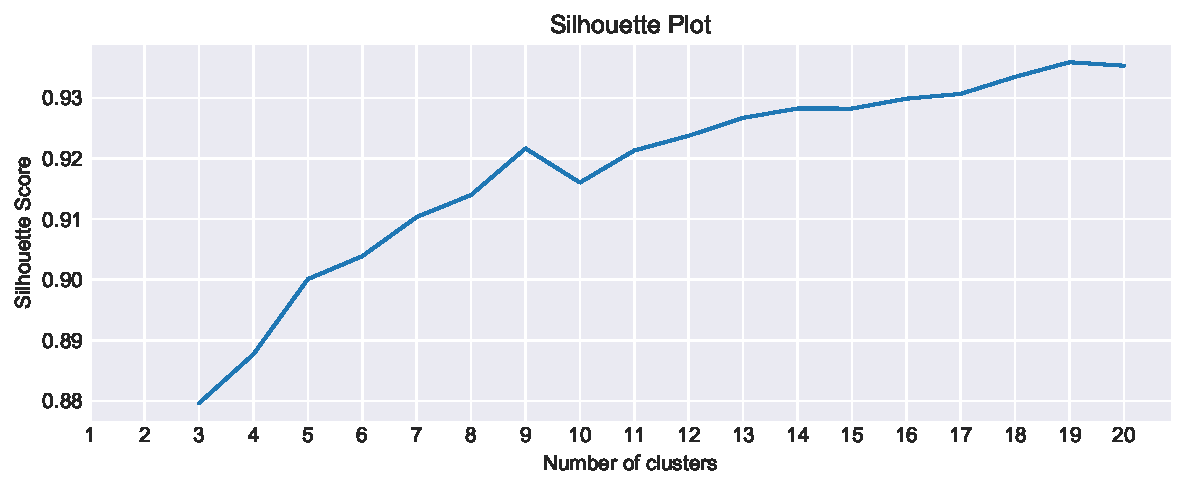
\includegraphics{figures/silhouette}
} \caption{The Silhoette score with varying number of clusters.} \label{fig:silhouette} \end{center} \end{figure} %

Figure~\ref{fig:silhouette} illustrates how the \textit{silhouette score} varies as the number of clusters is incremented up to 20. Although the is no completely clear choice, approximately 5 clusters is appropriate because the Silhouette score begins to plateau. With 5 clusters the score of $S\approx0.9$ is close to 1 which indicates high differentiation. Figure~\ref{fig:cluster_profiles} illustrates how the values of each of the factors in Table~\ref{tab:cluster_features} varies by each cluster. 

\begin{figure}[ht] \begin{center} 
\resizebox{0.9\textwidth}{!}{ 
	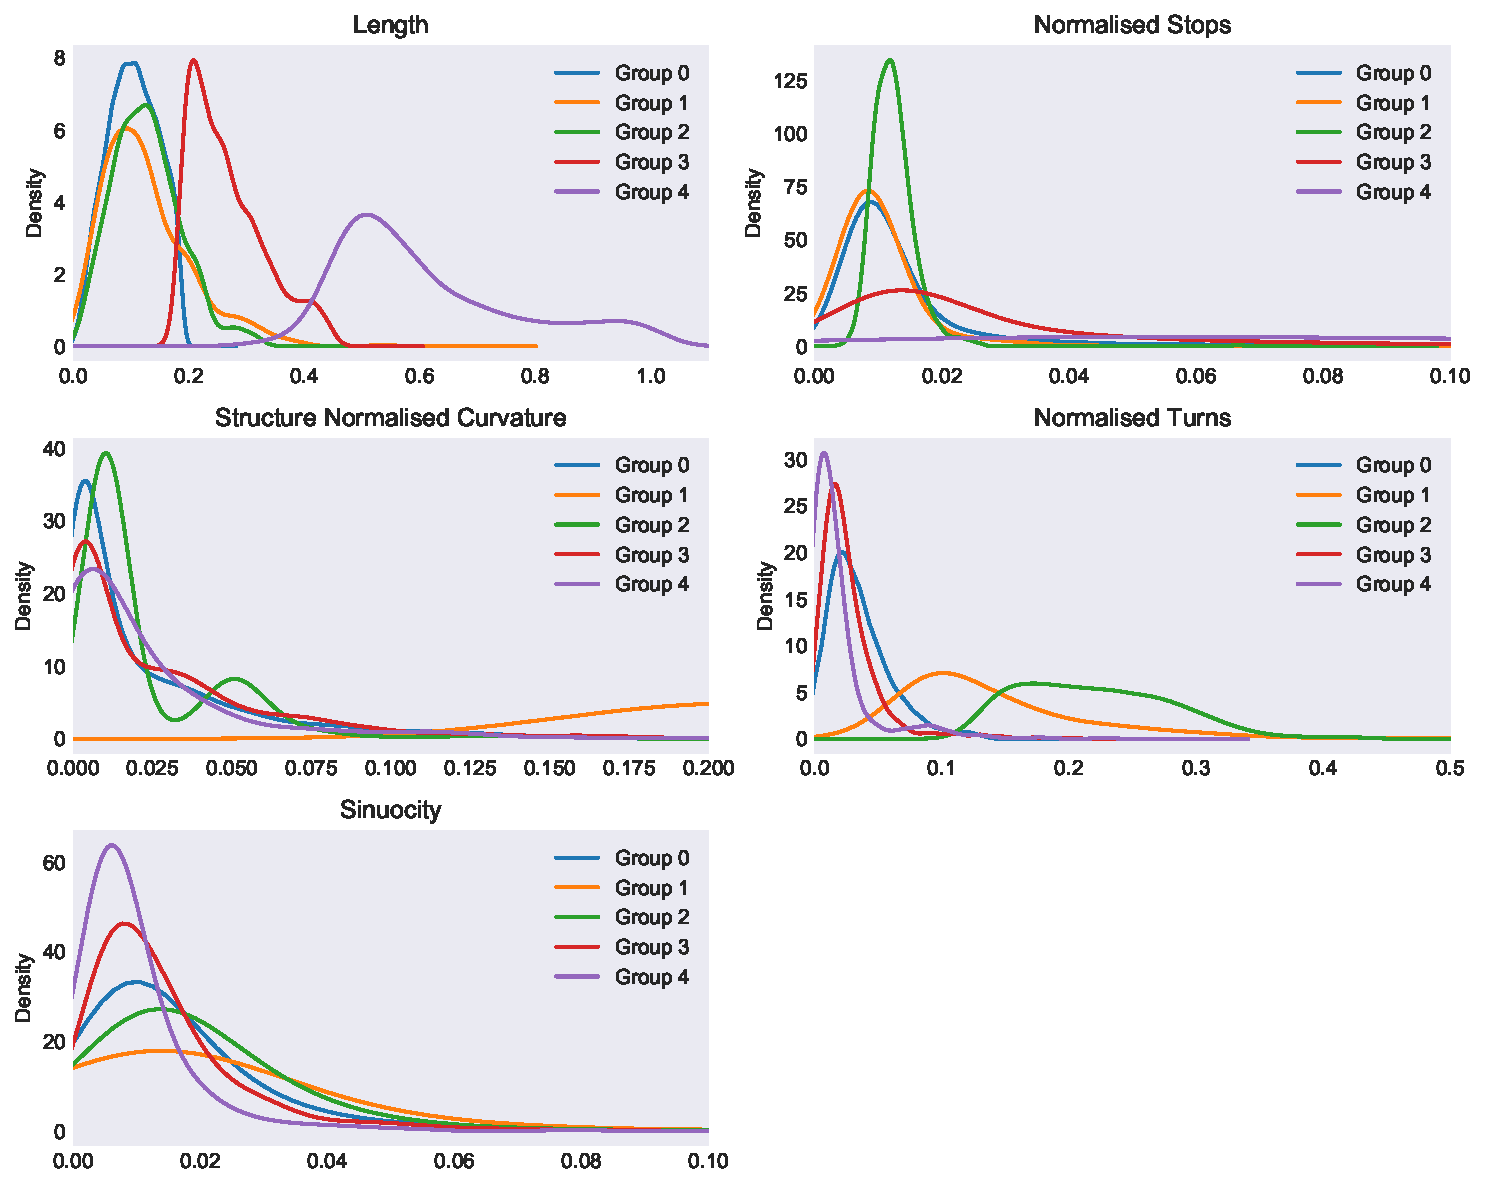
\includegraphics{figures/cluster_profiles}
} \caption{Cluster profiles.} \label{fig:cluster_profiles} \end{center} \end{figure} %

The next stage in the research will be to begin to label and further analyse the clusters. In particular, it will be interesting to begin to compare different city structures in different countries to see whether the local bus routes share similar characteristics. To this end, Figure~\ref{fig:barh} show, for a subset of all the cities, what proportion of the routes in the city correspond to each cluster. These patterns are potentially interesting. For example, some European cities such as Belgium, Austria and Italy contain routes that predominantly belong to Cluster 0. This cluster is notable for having relatively short routes with typical sinuosity. At the other end of the scale, cities such as Auckland, Washington DC, Toulouse and Budapest have very few Cluster 0 routes but many more Cluster 2 routes. Cluster 2 routes have very large numbers of stops and large numbers of turns compared to the other clusters. Like Cluster 0, Cluster 3 routes are common throughout our set of cities, being the longer and straighter routes with few stops. 

\begin{figure}[h] \begin{center} 
\resizebox{0.9\textwidth}{!}{ 
	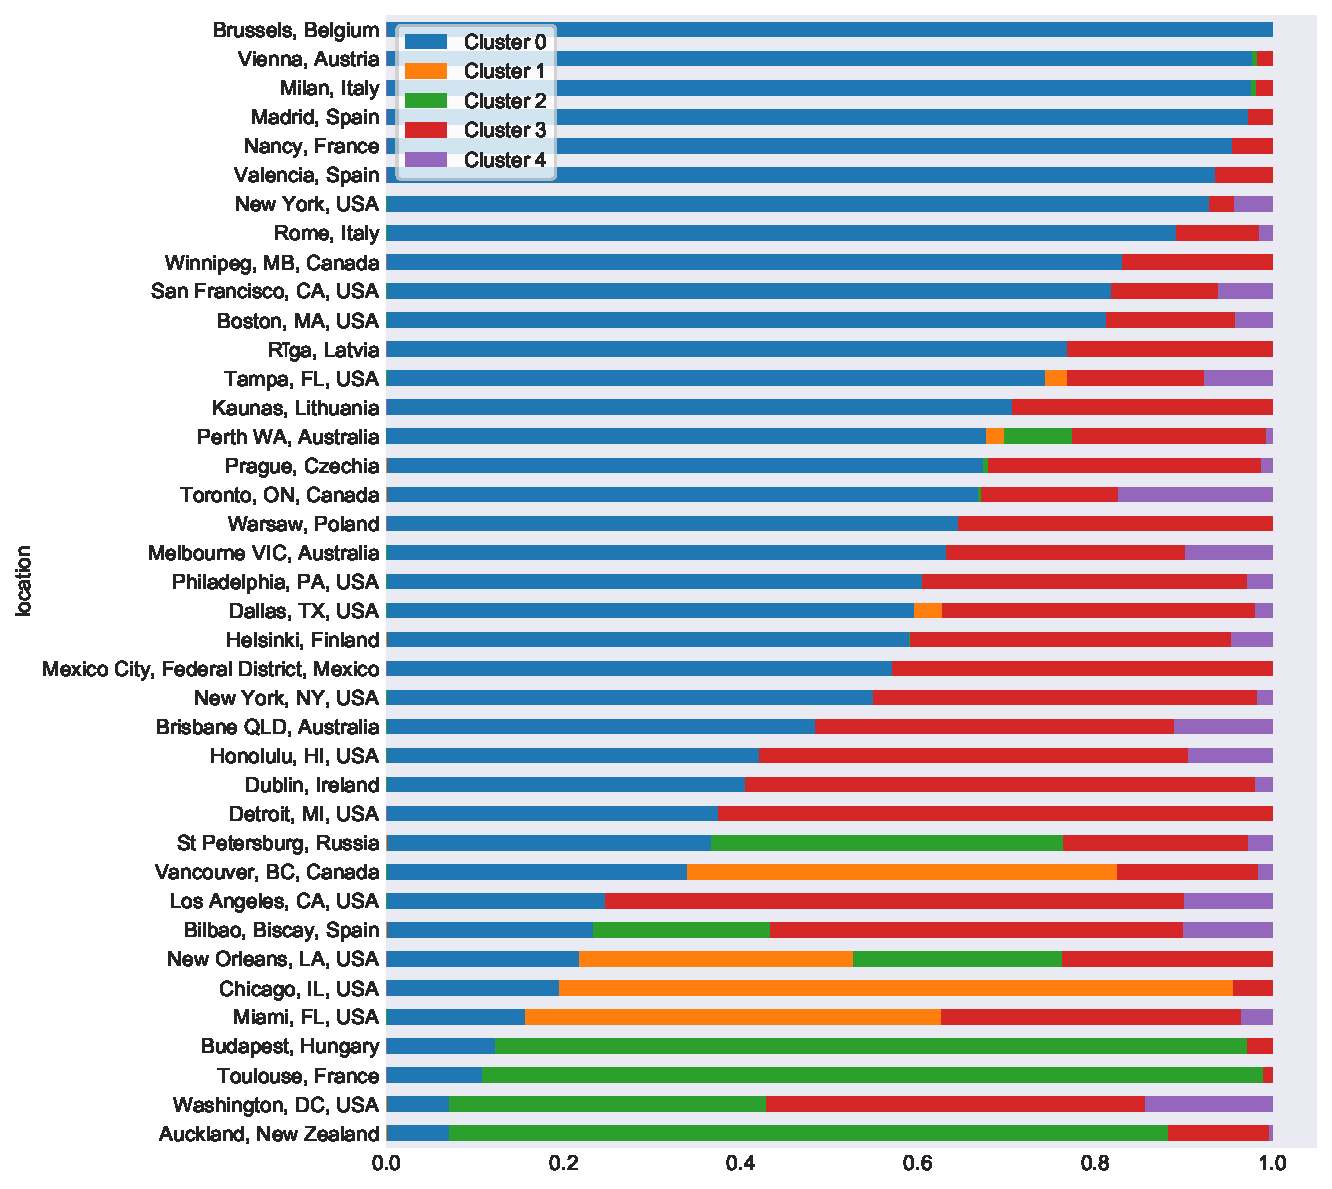
\includegraphics{figures/barh}
} \caption{Proportions of different route types within a subset of cities} \label{fig:barh} \end{center} \end{figure} %

While this initial analysis is not yet sufficiently advanced to make any firm statements about the approaches taken by different national or regional jurisdictions to their bus transport planning, it provides a useful basis for international comparison and measuring the effect of bus route design on outcomes.


\section{Conclusions} \label{conclusion}

This paper has demonstrated how General Transit Feed Specification (GTFS) data, that are published globally by a growing number of national and regional governments, can be combined with Open Street Map data to allow international comparisons of the structures of different bus routes. Clusters of routes were created and some preliminary analysis of these was conducted. Ultimately these data hold promise as a means of estimating the quality of bus service provision in global cities.



\section*{Biographies}

\textbf{Ed Manley} is Professor of Urban Analytics in the School of Geography, University of Leeds, and Turing Fellow at the Alan Turing Institute for Data Science and Artificial Intelligence. Ed's research aims to deepen our quantitative understanding of human behaviour in cities, and how these behaviours shape urban dynamics. He is author of the book `Agent-based Modelling and Geographical Information Science', recently published by Sage, Associate Editor of the Applied Spatial Analysis and Policy journal, and chairs the GIScience Research Group at the Royal Geographical Society.

\textbf{Steven Gray} is a Principal Teaching Fellow and a Spatial Software Engineer in the Centre for Advanced Spatial Analysis, University College London. As a Computing Scientist at heart,  Steve's research focuses on Large scale data collection, distributed systems (within the cloud) and data analysis, Human Computer Interaction, mobile development,, Web based Mapping and Ubiquitous Computing.  With over 20 years' professional software development under his belt, he has built multiple award-winning systems and his work has been featured in various worldwide media outlets.

\textbf{Nick Malleson}  is a Professor of Spatial Science at the Centre for Spatial Analysis and Policy at the School of Geography, University of Leeds, UK. He has a PhD in Geography and undergraduate degrees in Computer Science (BSc) and Multidiciplinary Informatics (MSc). Most of his research focuses on the development of computer models that help to understand and explain social phenomena. He has a particular interest in simulations of crime patterns, and in models that can be used to describe the flows of people around cities. More recently, he has become in interested in how `big' data, agent-based modelling, and smart cities initiatives can be used to better understand the daily dynamics of cities and reduce the impacts of phenomena such as pollution or crime.



% **************  REFERENCES **************

\bibliographystyle{apa}
\bibliography{references.bib}

\end{document}
